\chapter{Entfallende MSCs}

\section{Authentifizierung und Verschlüsselung} \label{hdl:grundlagen_aka}

\todo[inline]{wie wird überprüft ob der security context noch gültig ist und wo (VLR?)}
\todo[inline]{wie oft wird der security context gewechselt?}
\todo[inline]{cool wäre mitschnitt von laufendem gespräch}

\acused{RAND}\acused{XRES}\acused{Kc}\acused{Ki}\acused{SRES}

Für die Nutzung der meisten Funktionen des Netzwerks wird eine Authentifizierung vorausgesetzt. \citepauthor[3.2.3]{3gpp:02.09}Die Authentifizierung ist ein Ablauf im \ac{MM} und benötigt eine bestehende \ac{RR}-Verbindung, welche die direkte Kommunikation zwischen \ac{MS} und \ac{MSC} ermöglicht. Während einer \ac{RR}-Verbindung muss das \ac{MS} jederzeit  auf eine Authentifizierungsanfrage reagieren können. Authentifizierung wird immer vom \ac{VLR} gestartet, welches zuerst den Security Context des Netzteilnehmers anhand seiner \ac{IMSI} beim \ac{HLR} abfrägt [\textbf{1}] und speichert. Das \ac{HLR} lässt vom \ac{AuC} die Werte \ac{RAND}, \ac{XRES} und \ac{Kc} berechnen, in die der zur \ac{IMSI} passende \ac{Ki} mit einfließt und liefert diese über \ac{MAP} ans \ac{VLR} des \ac{MSC} zurück [\textbf{2}]. Mit dem erhaltenen Zufallswert \ac{RAND} wird die Challenge des \ac{GSM}-\ac{AKA} gebildet und als AUTHENTICATION-REQUEST ans \ac{MS} geschickt [\textbf{3}]. Dieses lässt vom \ac{SIM}, welches ebenfalls Zugriff auf den geheimen Schlüssel des Netzteilnehmers hat den zur Challenge passenden Security Context berechnen. Die \ac{SRES} wird in der Antwort ans \ac{MSC} zurückgegeben [\textbf{4}], das die Übereinstimmung von \ac{XRES} und \ac{SRES} überprüft. Da der Netzteilnehmer \ac{SRES} nur berechnen kann wenn er Zugriff auf \ac{Ki} hat, ist der Netzteilnehmer erfolgreich authentifiziert wenn \ac{XRES} === \ac{SRES}. In der Regel wird anschließend gleich dem \ac{BSS} über Cipher Mode Control \citepauthor[3.1.14]{3gpp:08.08} der Security Context ausgeliefert, wie in \autoref{fig:ciphering}[\textbf{1,2,3}] dargestellt. Damit die Authentifizierung nicht für jeden Layer 3 Service wie zum Beipiel einen Anruf neu durchlaufen werden muss, wird vom \ac{MSC} für den vom HLR erhaltenen Security Context die \ac{CKSN} vergeben. Das \ac{MS} erhält diese im AUTHENTICATION-REQUEST. \citepauthor[4.3.2.4, 10.5.1.2]{3gpp:24.008} Anhand dieser kann das \ac{VLR} feststellen, ob die \ac{Kc} von \ac{BTS} und \ac{MS} noch konsistent sind. Falls die \ac{CKSN} übereinstimmen, wird die Authentifizierung übersprungen und der im Security Context gespeicherte \ac{Kc} verwendet. \citepauthor[4.3.2]{3gpp:24.008}

\begin{figure}[H]
  \begin{center}
    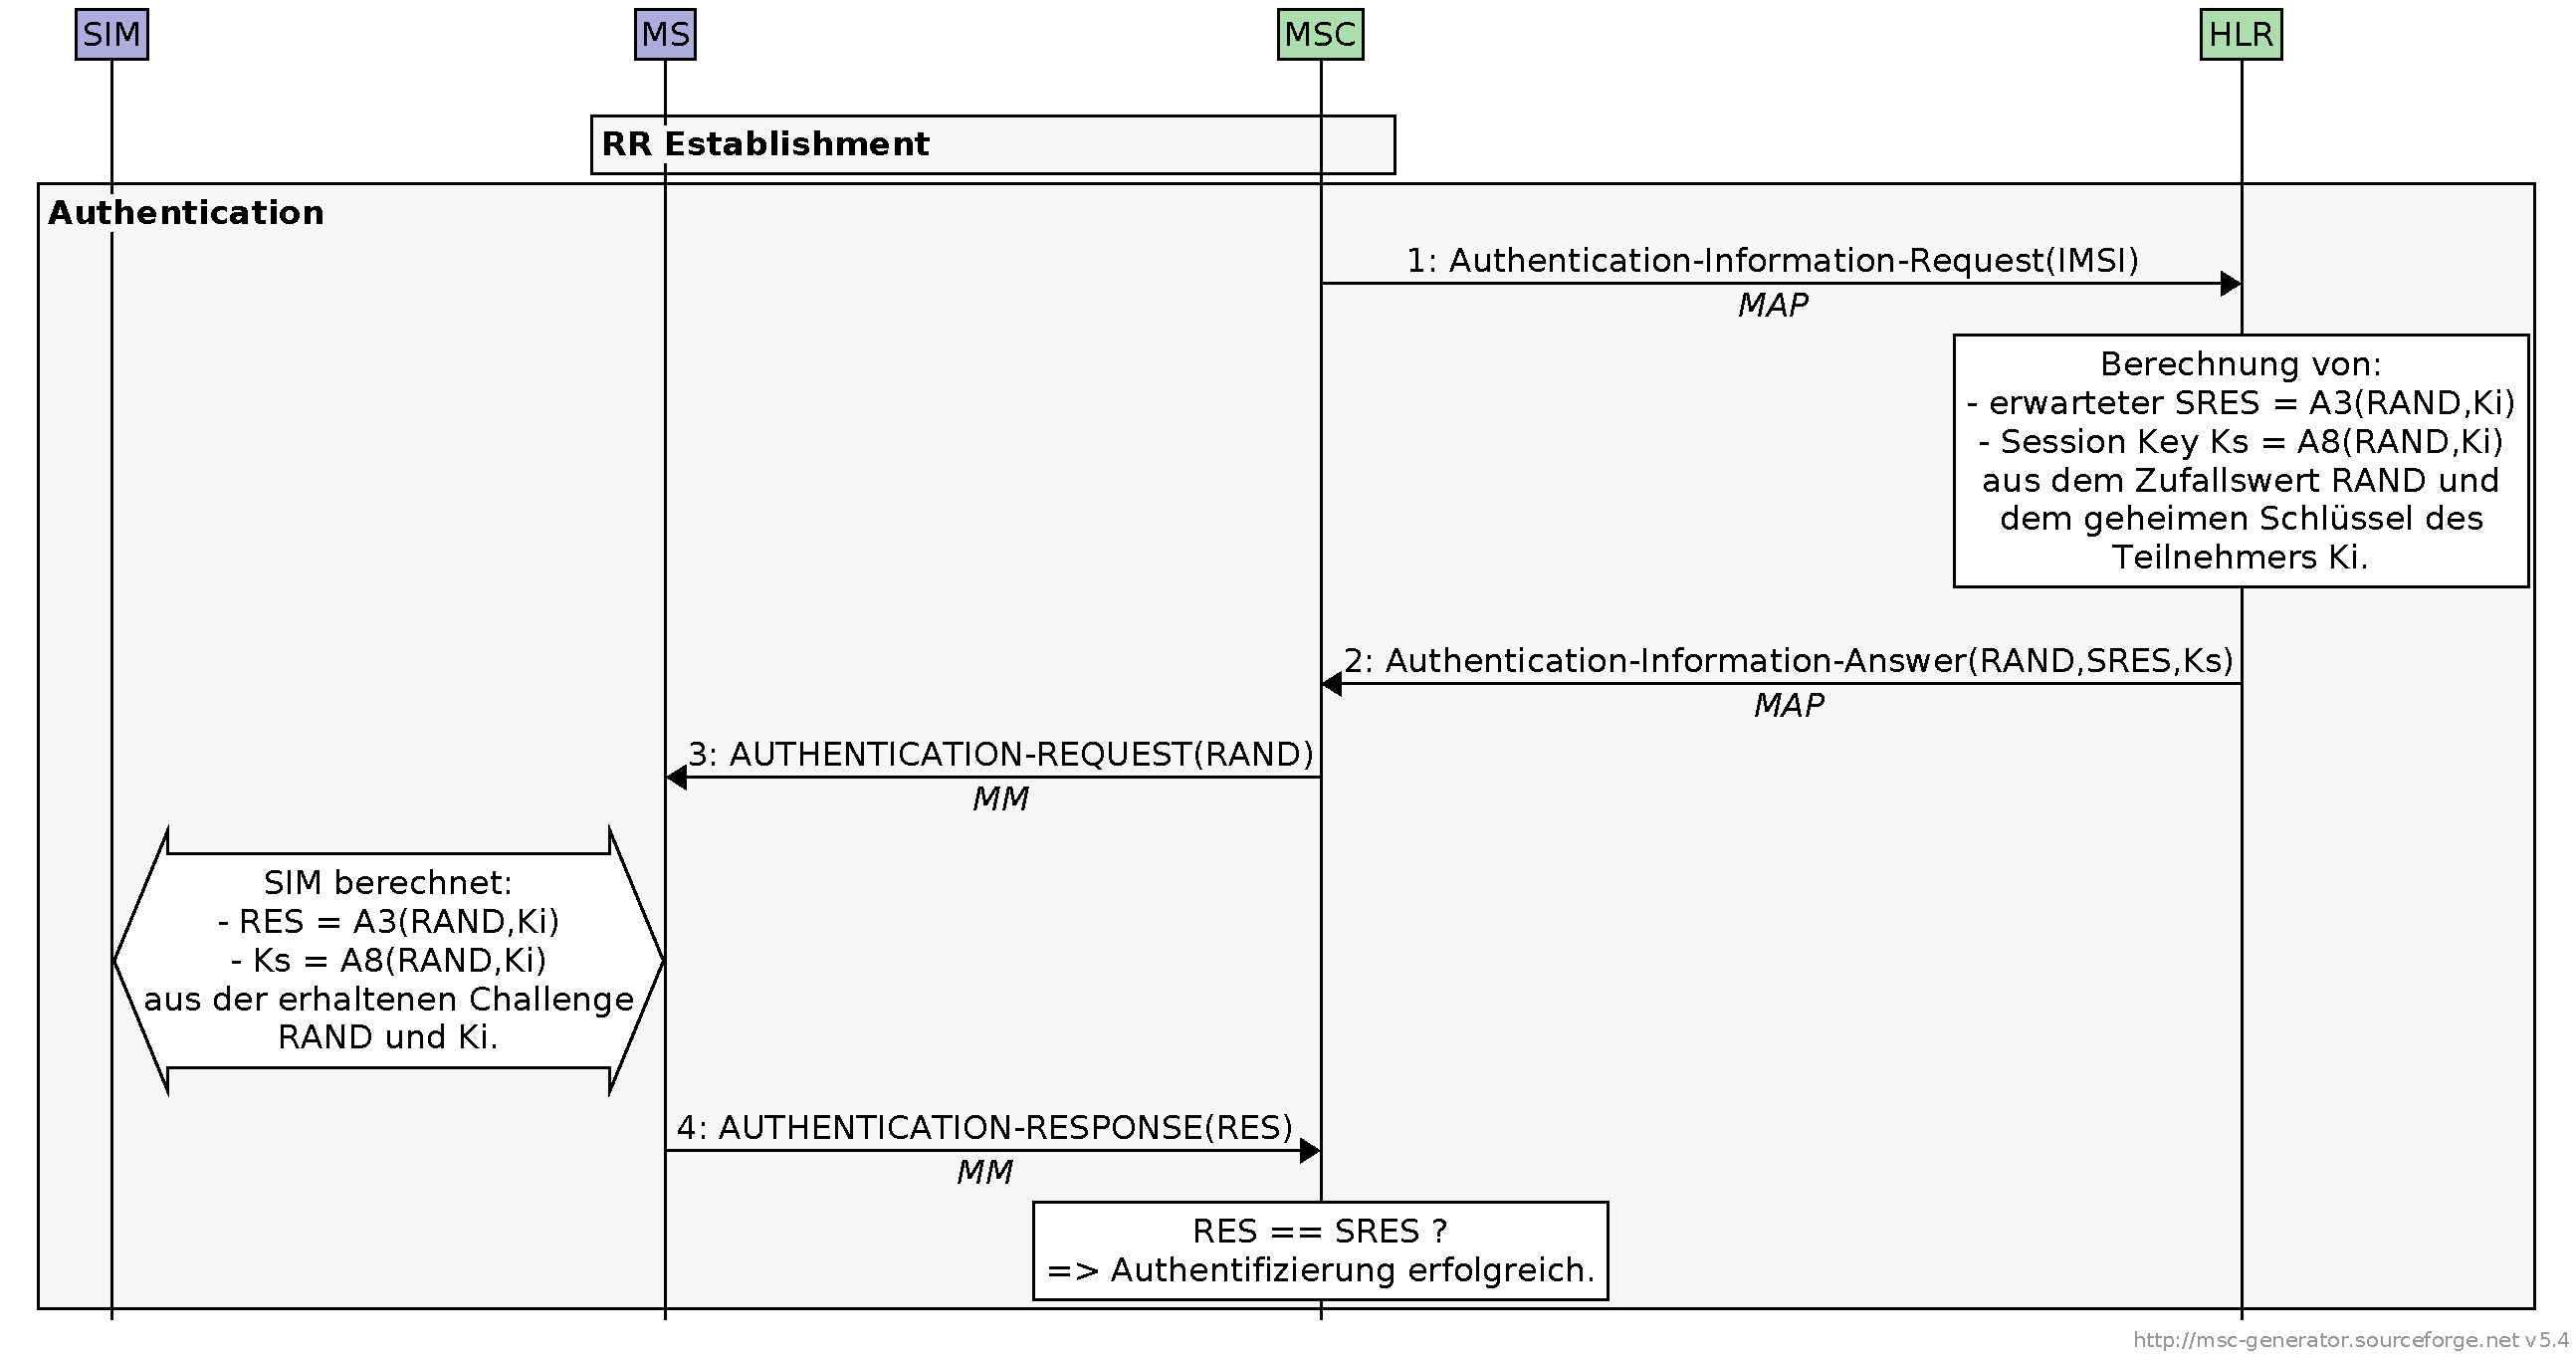
\includegraphics[width=1.00\textwidth]{figures/gsm_authentication.pdf}
  \end{center}
  \caption[Authentifizierung eines Mobilfunkteilnehmers]{Authentifizierung eines Mobilfunkteilnehmers} \label{fig:authentication}
\end{figure}

Das Einrichten einer verschlüsselten Verbindung ist eine \ac{MM} Prozedur und setzt sowohl eine eingerichtete \ac{RR}-Verbindung als auch einen bestehenden Security Context zwischen Netzteilnehmer und Netzwerk voraus (siehe \autoref{fig:ciphering}). Mit dem CIPHER-MODE-CMD aktualisiert das \ac{MSC} die im \ac{BSS} gespeicherten Verschlüsselungsinformationen zu einem \ac{MS} [\textbf{1}]. Der Befehl enthält für das \ac{BSS} erlaubte Verschlüsslungsalgorithmen (A5/0-A5/7) sowie den Schlüssel \ac{Kc} des Security Contexts. \citepauthor[3.2.1.30]{3gpp:08.08} 
\citepauthor[3.2.1.30]{3gpp:08.08} Der \ac{BSC} leitet die erhaltenen Informationen im ENCRYPTION-CMD an den \ac{BTS} weiter und gibt ihm damit auch den Befehl, die Verschlüsselung für die aktuelle Verbindung zu starten [\textbf{2}]. \citepauthor[4.4]{3gpp:08.58} Als eine der wenigen nicht-transparenten Nachrichten (\citepauthor[8.1]{3gpp:08.58}) wird ENCRYPTION-CMD im \ac{BTS} bearbeitet. Er speichert den Schlüssel \ac{Kc} ab, wählt den sichersten \ac{BSS} und \ac{MS} kompatiblen Algorithmus aus und startet Entschlüsselung auf dem Uplink. Mit einer CIPHERING-MODE-CMD Nachricht wird dem \ac{MS} mitgeteilt, dass dieser Kanal ab jetzt verschlüsselt wird und mit welchem Algorithmus [\textbf{3}]. \citepauthor[9.1.9]{3gpp:04.18} Das \ac{MS} startet daraufhin Verschlüsselung auf Up- und Downlink mit dem aus dem Authentifizierungsverfahren gespeicherten Schlüssel \ac{Kc} und antwortet dem \ac{BTS} mit einer bereits verschlüsselten CIPHERING-MODE-COMPLETE Nachricht [\textbf{4}]. Kommt diese beim \ac{BTS} an, beginnt er mit der Verschlüsselung auf dem Downlink und signalisiert \ac{BSC} -- welcher die Nachricht gleich ans \ac{MSC} weiterleitet -- dass der CIPHER-MODE-CMD ausgeführt wurde [\textbf{5,6}].

\begin{figure}[H]
  \begin{center}
    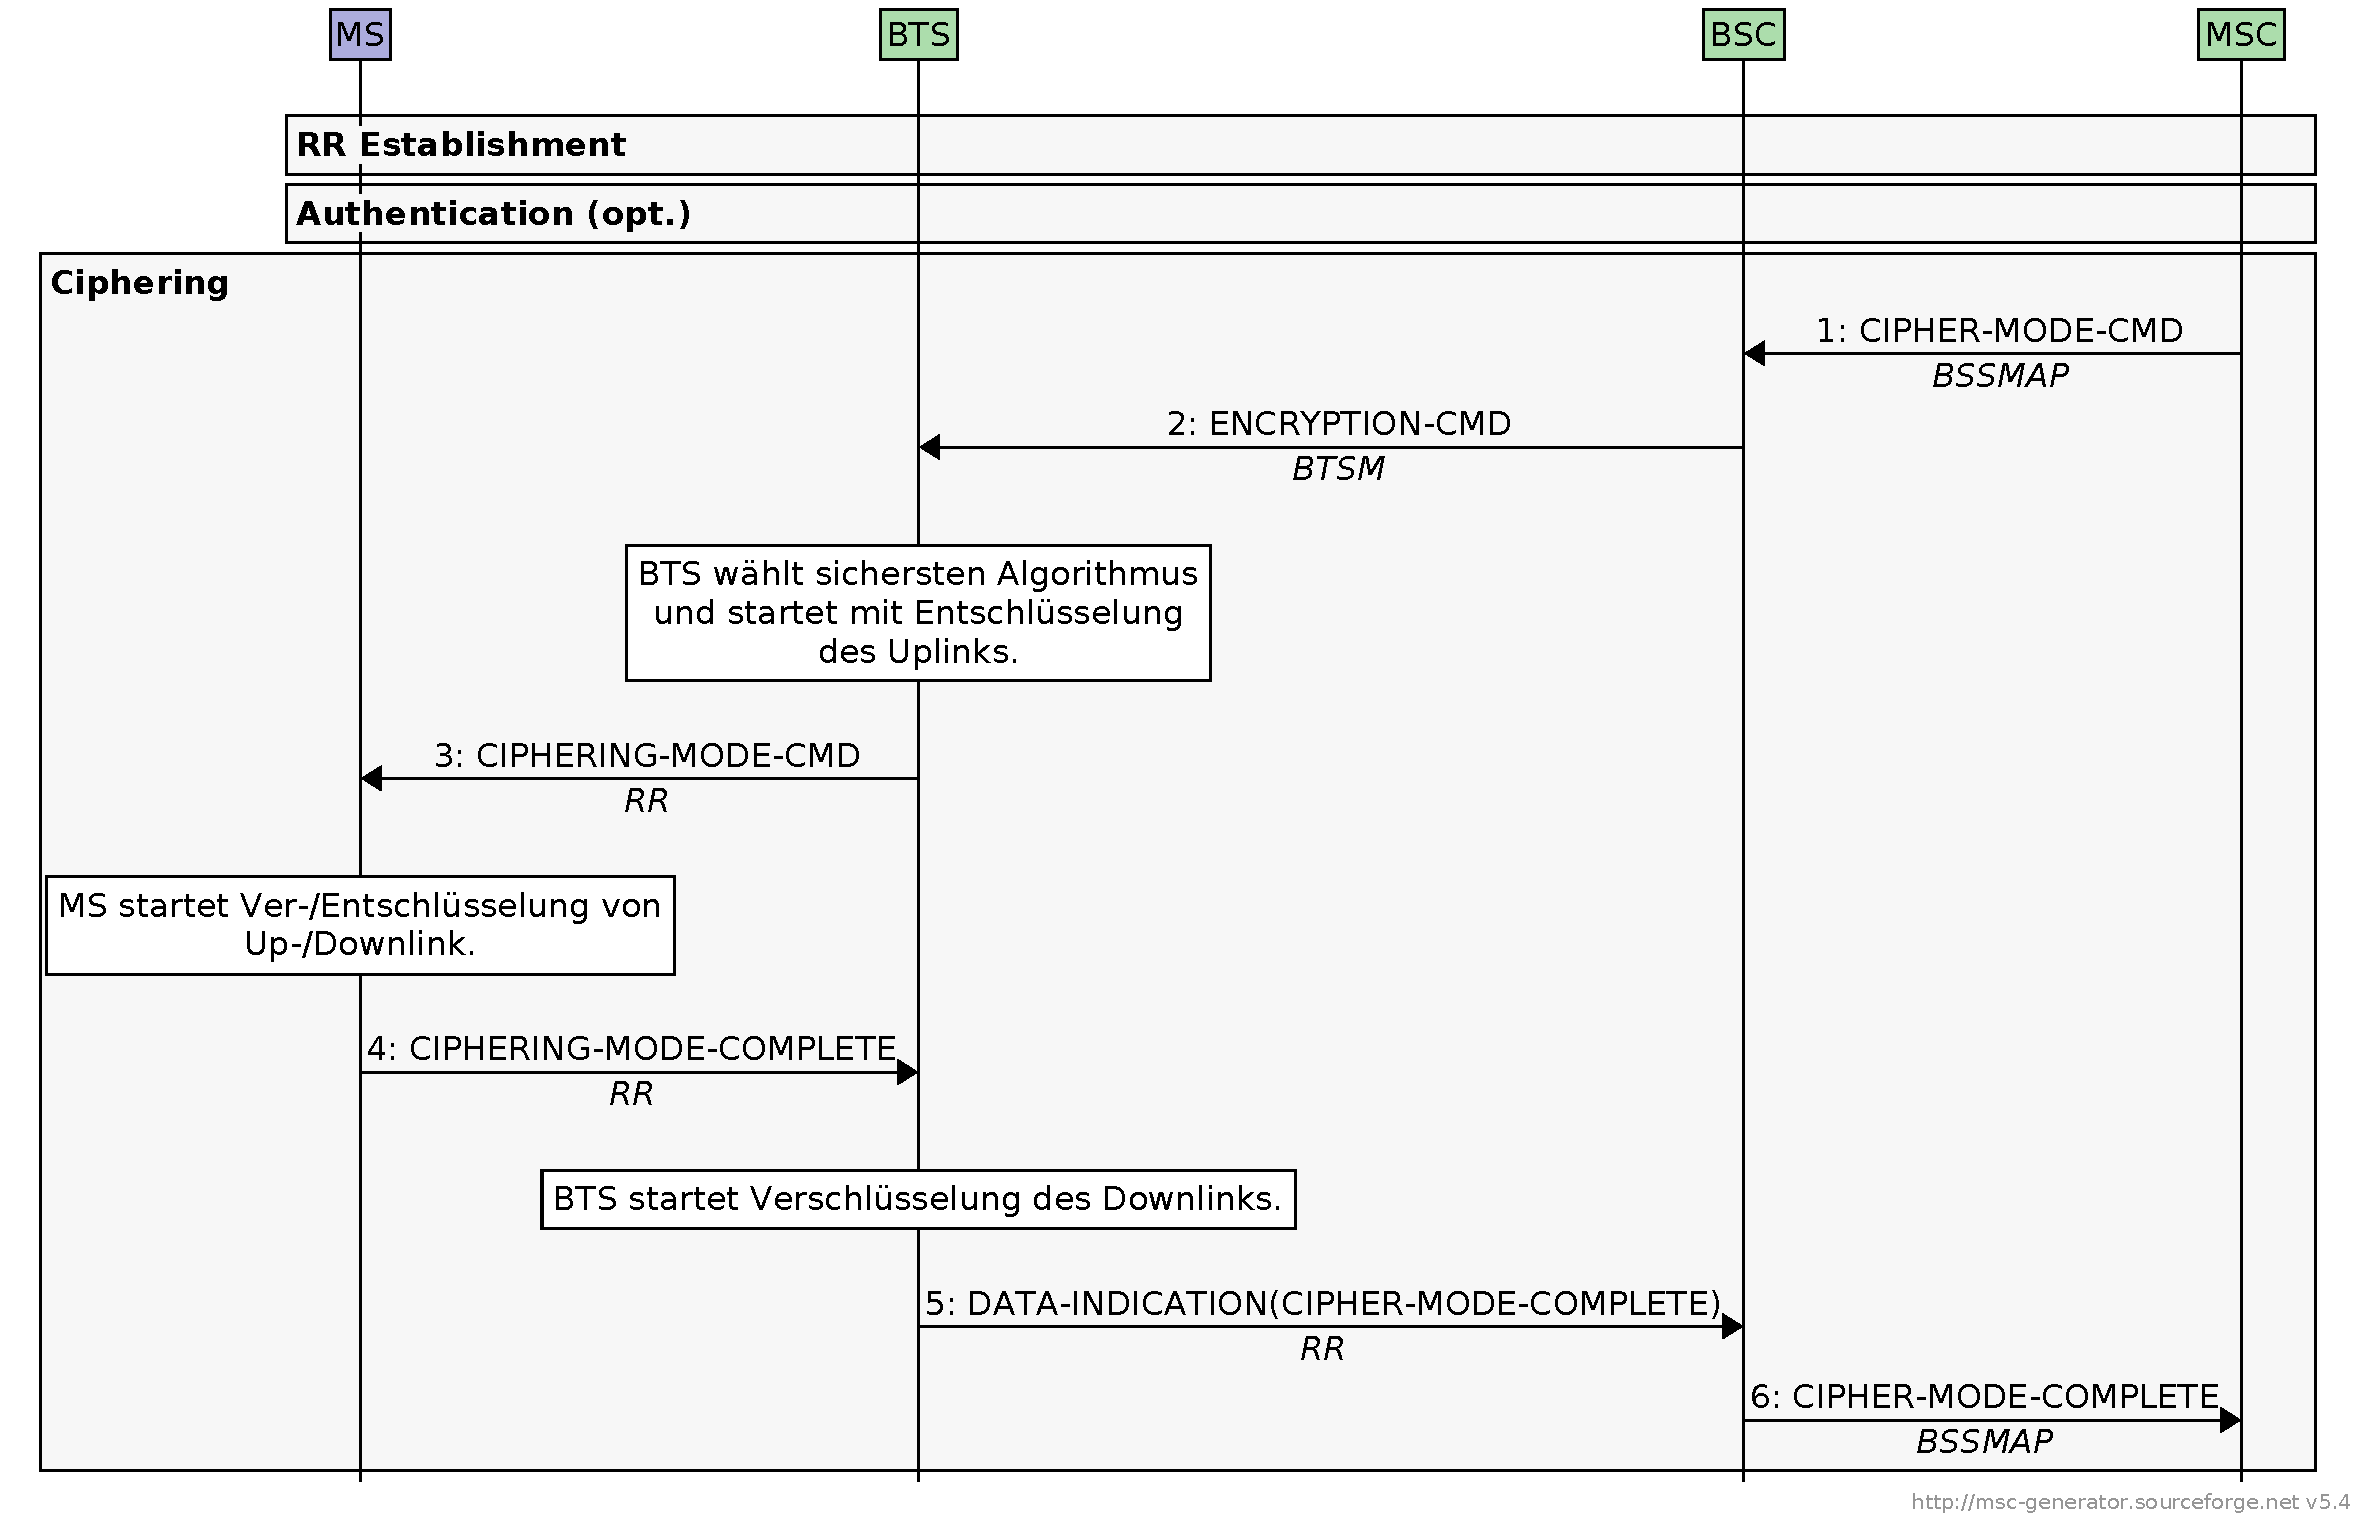
\includegraphics[width=1.00\textwidth]{figures/gsm_ciphering.pdf}
  \end{center}
  \caption[Einrichten eines verschlüsselten Kanals]{Einrichten eines verschlüsselten Kanals} \label{fig:ciphering}
\end{figure}

\section{Mobile originated Call Establishment} \label{hdl:grundlagen_ablufe}

\todo{Call Setup Message!}

% Search call establishment in pcaps:
% * All Call Control Messages:
%   gsma.dtap.protocoldiscriminator==0x03 
%   oder gsm_a.dtap.msg_cc_type
% * Call Control Message type == SETUP
%   gsm_a.dtap.protocol_discriminator==0x03
%   || gsm_a.dtap.msg_cc_type==0x05
% * Assignment CMD messages
%   gsm_a.dtap.msg_rr_type==0x2e
% In the pcap file from 44CON, there are some procedures recorded. 13992 and 13999 seem to be retransmissions!

%\citepauthor[7.3.2]{3gpp:23.108} - Mobile originating call (Stage 2)
%\citepauthor[5.2.1]{3gpp:24.008} - Mobile originating call (Stage 3)
%\citepauthor[A.1, Scheme 5+6]{3gpp:43.020} - Mobile originating call , Security Aspects
%\citepauthor[5.1]{3gpp:23.018}  - Mobile originating call, information flow
%\citepauthor[9.3.23.2]{3gpp:24.008} - Setup Message
%\citepauthor[3.4.3.1]{3gpp:04.18} Assignment

Der in \autoref{fig:moc} aufgeführte \ac{MOC} ist der Ablauf, in den bei unserem Angriff eingegriffen wird. Um jemanden anrufen zu können, muss zuerst eine \ac{RR}-Verbindung eingerichtet werden. Da die Routine der \acl{CC} des \acl{CM} zugeordnet ist, wird diese mit einem CM-SERVICE-REQUEST als Parameter initialisiert. Der Service Request enthält u.a. die \ac{CKSN}, mit der überprüft wird, ob Authentifizierung notwendig ist. \citepauthor[9.2.9]{24.008} Bei übereinstimmenden \ac{CKSN} von Netzwerk und \ac{MS} muss die Authentifizierungsprozedur nicht ausgeführt werden, sondern kann direkt die Verschlüsselung eingeleitet werden. Im Anschluss wird Authentifizierung ausgeführt, falls noch kein Security Context für den Netzteilnehmer besteht und der reservierte Kanal verschlüsselt. Durch eine CM-SETUP Nachricht ans \ac{MSC} mit der Rufnummer des Empfängers wird der Anruf eingeleitet [\textbf{1}]. Nachdem das \ac{MSC} von seinem \ac{VLR} als Antwort auf eine \ac{SIFOC} Nachricht  zusätzliche Informationen zum ausgehenden Anruf erhalten hat, schickt es dem \ac{MS} ein CALL-PROCEEDING [\textbf{1}]. Das \ac{MS} weiss damit, dass der Anruf im Aufbau ist. Beim Early Assignment kümmert sich das \ac{BSS} direkt im Anschluss um die Reservierung eines \ac{TCH} für die Sprachübertragung [\textbf{3,4}]. \citepauthor[3.4.3.1]{3gpp:04.18} Es gibt auch noch die Varianten Very Early Assignment (siehe \autoref{hdl:grundlagen_rr-conn-est}) und Late Assignment, bei der der Kanal erst nach dem ALERTING [\textbf{7}] reserviert wird. Das MSC informiert die Zielvermittlungsstelle mit einer \ac{ISDN-UP} \ac{IAM} Nachricht über den ausgehenden Anruf [\textbf{5}]. Ist die Telefonnummer gültig und das Zieltelefon gefunden und alarmiert, wird diese mit einer \ac{ACM} Nachricht antworten [\textbf{5}]. Um dem \ac{MS} mitzuteilen, dass der Anruf durchgestellt wurde, schickt das \ac{MSC} eine ALERTING Nachricht ans \ac{MS}[\textbf{8}]. Wenn die angerufene Partei den Anruf beantwortet ("abhebt"), wird das MS über einen CONNECT Befehl aufgefordert, die Sprachverbindung durchzuleiten [\textbf{9,10}]. Die Verbindung bleibt solange erhalten bis einer der Gesprächspartner auflegt oder über längere Zeit keinen Empfang mehr hat. Die Verbindung kann durch den \ac{CC} DISCONNECT Befehl beendet werden. \citepauthor[5.1]{3gpp:23.018}, \citepauthor[7.3.2]{3gpp:23.108} \citepauthor[5.2.1]{3gpp:24.008}

\begin{figure}[H]
  \begin{center}
    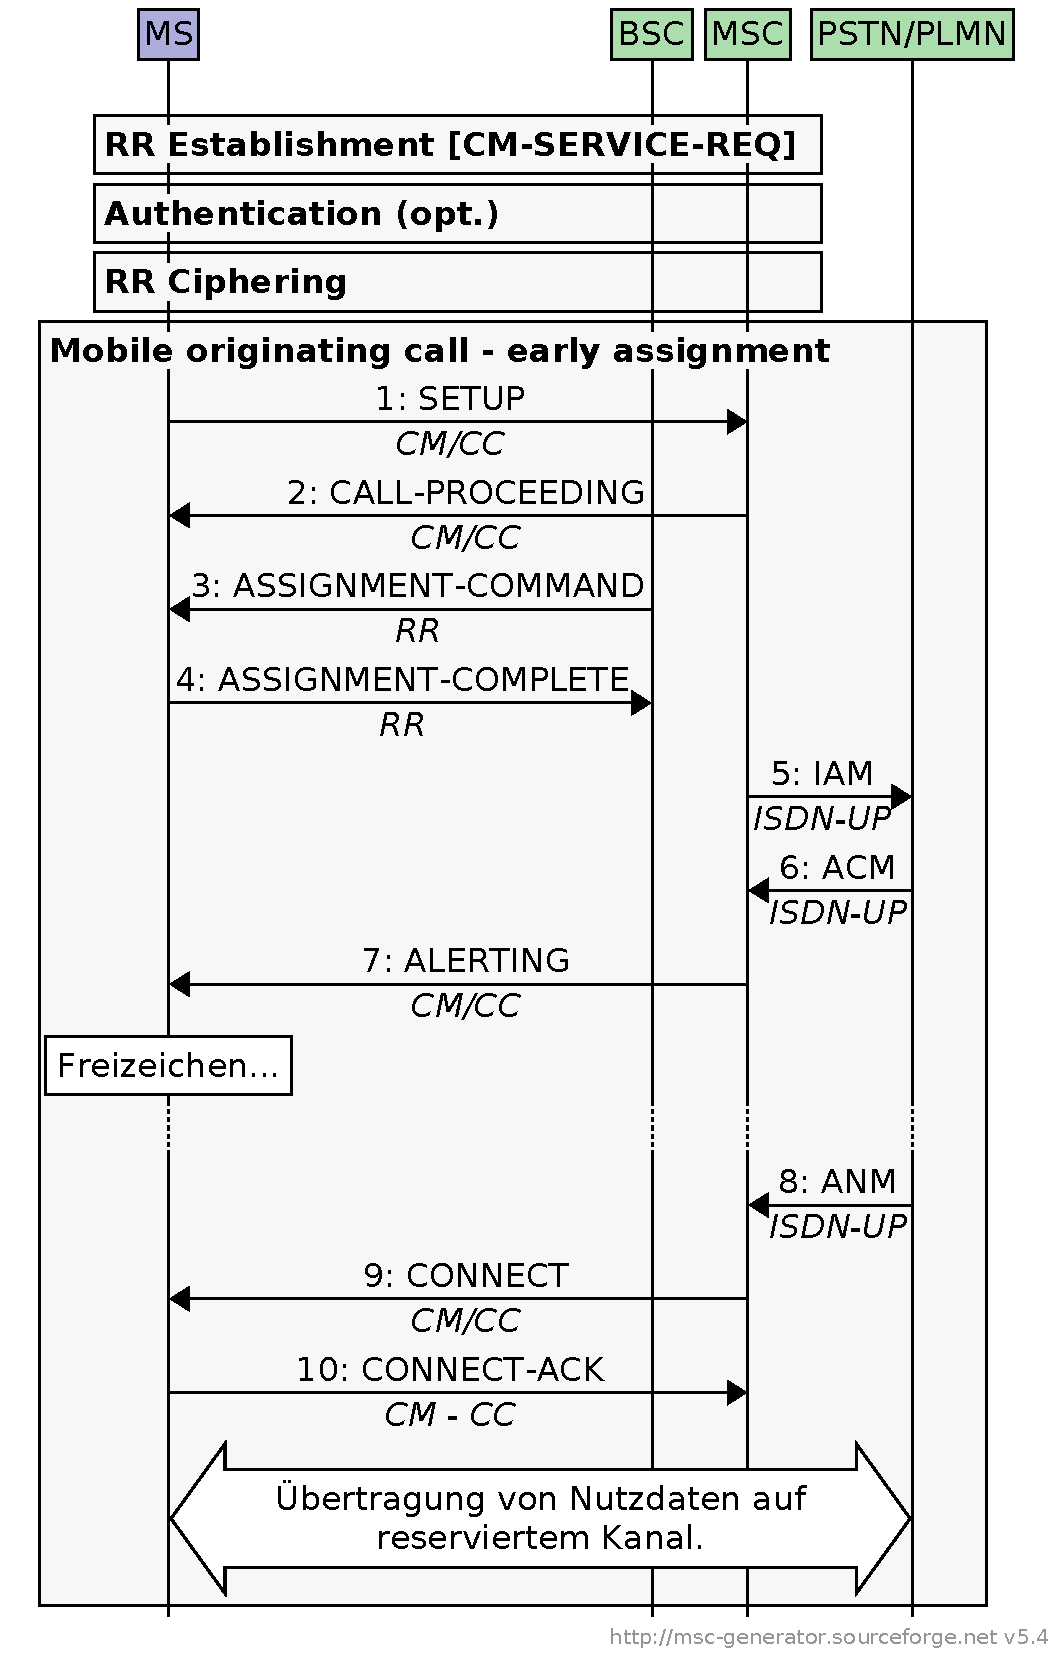
\includegraphics[width=0.5\textwidth]{figures/gsm_mobile_orig_call.pdf}
  \end{center}
  \caption[\ac{MOC}]{\ac{MOC}} \label{fig:moc}
\end{figure}

\citepauthor[11.2.5]{3gpp:24.007} - Presence Requirements
\citepauthor[11.2.1.1.4]{3gpp:24.007} - Formats
\citepauthor[11.2.3.1.1]{3gpp:24.007} - Protocol Discriminator (PD) [0011] = Call Control
\citepauthor[11.2.3.1.3]{3gpp:24.007} - Transaction Identifier (TI) [0XXX] = counter, hängt von den aktuell laufenden Transactions ab
\citepauthor[11.2.3.2]{3gpp:24.007}, \citepauthor[10.4]{3gpp:24.008} - Message type octet [00000101] = type:SETUP 
\citepauthor[10.5.4.22]{3gpp:24.008} Repeat Indicator - Conditional! Wird gesetzt, um mehrfach übermittelte Informationselemente anzuzeigen. Z.B. Bearer Capability 1 für Multimedia Call -- Bearer Capability 2 für Fallback Speech Call
\citepauthor[3.6]{3gpp:24.080}, \citepauthor[10.5.4.15]{3gpp:24.008}, 
\citepauthor[2.2.4.1.2]{3gpp:24.010} - Facility information element

Alle Informationselemente haben Identifier, die ihren typ festlegen. Ein Informationelement kann unterschiedlich formatiert sein! (s. Formats) \citepauthor[11.2.1.1.4]{3gpp:24.007}


Da das Wissen um den Aufbau der SETUP Nachricht essentiell für die vorgestellte \ac{MitM} Attacke ist, soll dieser im Folgenden beschrieben werden. \citepauthor[9.3.23.2]{3gpp:24.008}
\todo[inline]{Aufbau der SETUP Message}

\todo[inline]{MSISDN in Call Setup Message immer gleich lang?}
NEIN
\todo[inline]{Wie oft ist retransmission von Setup message möglich bis verbindungsaufbau abgebrochen wird?}
\todo[inline]{Falsche oder unbekannte tel??}
\todo[inline]{Verschlüsselungsproblem, Fehlerhafter Paritätscheck} geregelt über LAPDm Acknowledged Mode und Timer t200 (nach ablauf ohne erhalt von ack-retransmit frame) sowie n200 (max number of retransmissions) TS: 44.006-8.8.2.1: n200 = 23 for use on SDCCH; 5 for use on SACCH; t200= implementation dependent

\todo[inline]{Wird bei Retransmission der setup message der selbe Keystream verwendet oder wird die Nachricht neu verschlüsselt?}
Anderer Keystream, da die aktuelle FN in die Genereirung des Keystreams mit einfließt